\documentclass[10pt,a4paper, margin=1in]{article}
\usepackage{fullpage}
\usepackage{amsfonts, amsmath, pifont}
\usepackage{amsthm}
\usepackage{graphicx}
\usepackage{float}

\usepackage{tkz-euclide}
\usepackage{tikz}
\usepackage{pgfplots}
\pgfplotsset{compat=1.13}
\usetikzlibrary{positioning}


\begin{filecontents}{q3.dat}
 n   xn
 -1  1
 0   0
 1   0  
 2   -2
 3   0
 4   3 
 5   0
 6   0
 7   -4
\end{filecontents}


\begin{filecontents}{q31.dat}
 n   xn
 1  1
 0   0
 -1   0  
 -2   -2
 -3   0
 -4   3 
 -5   0
 -6   0
 -7   -4
\end{filecontents}

\begin{filecontents}{q32.dat}
 n   xn
 -1  1
 0   0
 1   0  
 2   0
 3   -4
\end{filecontents}

\begin{filecontents}{q3ans.dat}
 n   xn
 3 -4
 2 0
 1  1
 0   0
 -1   1  
 -2   -2
 -3   0
 -4   3 
 -5   0
 -6   0
 -7   -4
\end{filecontents}


\usepackage{geometry}
 \geometry{
 a4paper,
 total={210mm,297mm},
 left=10mm,
 right=10mm,
 top=10mm,
 bottom=15mm,
 }
 % Write both of your names here. Fill exxxxxxx with your ceng mail address.
 \author{ 
  Uçan, Yiğitcan\\
  \texttt{e2310555@ceng.metu.edu.tr}
  \and
  Akın, Ozan\\
  \texttt{e2309599@ceng.metu.edu.tr}
}
\title{CENG 384 - Signals and Systems for Computer Engineers \\
Spring 2021 \\
Homework 1}
\begin{document}
\maketitle


\noindent\rule{19cm}{1.2pt}

\begin{enumerate}

\item 

\[ e = \lim_{n\to0} (1+n)^{\frac{1}{n}} \]	

\[ \frac{d}{dx} e^x = \lim_{\Delta x\to 0} \frac{e^{x+\Delta x} - e^x}{\Delta x} \]	

\[ \frac{d}{dx} e^x = e^x \cdot \lim_{\Delta x\to 0} \frac{e^{\Delta x} - 1}{\Delta x} \]	

Some replacements for $\Delta x$ below. Also note that as $\Delta x\to 0$, $n\to 0$.

\[n = e^{\Delta x} - 1\ \ \ \  n + 1 = e^{\Delta x}\ \ \ \  ln(n+1) = \Delta x \]

\[ \frac{d}{dx} e^x = e^x \cdot \lim_{\Delta n\to 0} \frac{n}{ln(1+n)} \]

\[ \frac{d}{dx} e^x = e^x \cdot \lim_{\Delta n\to 0} \frac{1}{\frac{1}{n} \cdot ln(1+n)} \]	

\[ \frac{d}{dx} e^x = e^x \cdot \lim_{\Delta n\to 0} \frac{1}{ln((1+n)^\frac{1}{n})} \]

\[ \frac{d}{dx} e^x = e^x \cdot \frac{1}{ln(\lim_{\Delta n\to 0} (1+n)^\frac{1}{n})} \]

Using the definition we have written at the beginning we can prove that $e^x$'s derivative equal to itself.

\[ \frac{d}{dx} e^x = e^x \cdot \frac{1}{ln(e)} \]

\[ \frac{d}{dx} e^x = e^x \]	


\item %write the solution of q2
    \begin{enumerate}
    % Write your solutions in the following items.
    \item 
        \[ z = x + jy, \bar {z} = x - jy \]
        \[ z - 3 = j - 2 \bar {z} \]
        \[ z - 3 - j = - 2 \bar {z} \]
        \[ x + jy - 3 - j = - 2 (x - jy) \]
        \[ x + jy - 3 - j = -2x + 2jy \]
        \[ 3x - jy = j + 3 \]
        \[ x = 1, y = -1 \]
        
\newpage
        
        \begin{enumerate}
            \item $|z|^2 = x^2 + y^2 = 1^2 + (-1)^2 = 2$
            \item ~ \\
            
            \begin{tikzpicture}
                \begin{scope}[thick,font=\scriptsize]
                    \draw [->] (-4,0) -- (4,0) node [above left]  {$\Re\{z\}$};
                    \draw [->] (0,-4) -- (0,4) node [below right] {$\Im\{z\}$};
                    
                    \foreach \n in {-3,-2,-1,1,2,3}{%
                        \draw (\n,-3pt) -- (\n,3pt)   node [above] {$\n$};
                        \draw (-3pt,\n) -- (3pt,\n)   node [right] {$\n$};
                    }
                        
                    \draw [thick, color=black] (0,0) -- (1,-1);
                    \draw [color=black, fill=black] (1,-1) circle(0.05);
                    \node [color=black] at (1,-1.3) {$      1-j$};
                \end{scope}
            \end{tikzpicture}
        \end{enumerate}
            
    \item 
        \[ z^4 = -81 \]
        \[ z^4 + 81 = (z^2 + 9j) \cdot (z^2 - 9j) = 0 \]
        \[ z^2 = 9j \; \text{or} \; z^2 = -9j \]
        
        ~ \\
        \[ z^2 = (a + bj)^2 = 9j \]
        \[ (a^2 - b^2) + 2abj = 0 + 9j \]
        \[ a = b, 2ab = 9, ab = \frac{9}{2} \]
        \[ a = b = \frac{3\sqrt{2}}{2}  \]
        ~ \\
        \[ z^2 = (a + bj)^2 = -9j \]
        \[ (a^2 - b^2) + 2abj = 0 + -9j \]
        \[ a = b, 2ab = -9, ab = \frac{-9}{2} \]
        \[ \text{Since $a = b$, $ab$ cannot be negative} \]
        ~ \\
        \[ r = \sqrt{a^2 + b^2} = \sqrt{\frac{9}{2} + \frac{9}{2}} = \frac{3}{2} \]
        \[ \frac{b}{a} = tan(\theta), \theta = \frac{\pi}{4} \]
        
        \[ z = \frac{3}{2} \cdot (cos(\frac{\pi}{4}) + j \cdot sin(\frac{\pi}{4})) \]
        
    \item 
        \[ z = \frac{(\frac{1}{2} + \frac{1}{2}j)(1-j)}{1 - \sqrt{3}j} \]
        \[ z = \frac{\frac{1}{2} - \frac{1}{2}j + \frac{1}{2}j + \frac{1}{2}}{1 - \sqrt{3}j} \]
        \[ z = a + bj = \frac{1}{4} + \frac{\sqrt{3}j}{4} \]
        \[ a = \frac{1}{4}, b = \frac{\sqrt{3}}{4} \]
        ~ \\
        \[ r = \sqrt{a^2 + b^2} = \sqrt{\frac{1}{16} + \frac{3}{16}} = \frac{1}{2}\]
        \[\ \theta = tan^{-1}(\frac{b}{a}) = tan^{-1}(\frac{\frac{\sqrt{3}}{4}}{\frac{1}{4}}) = tan^{-1}(\sqrt{3}) = \frac{\pi}{3}\]
    
    
    \item 
        \[ z = -\frac{3}{j} \cdot e^{j\pi / 2} \]
        \[ r = -\frac{3}{j}, \theta = \frac{\pi}{2} \]
        \[ z = -\frac{3}{j} \cdot (cos(\frac{\pi}{2}) + j \cdot sin(\frac{\pi}{2})) \]
    
    \end{enumerate}

\item Q3\\

\begin{figure}[h!]
    \centering
        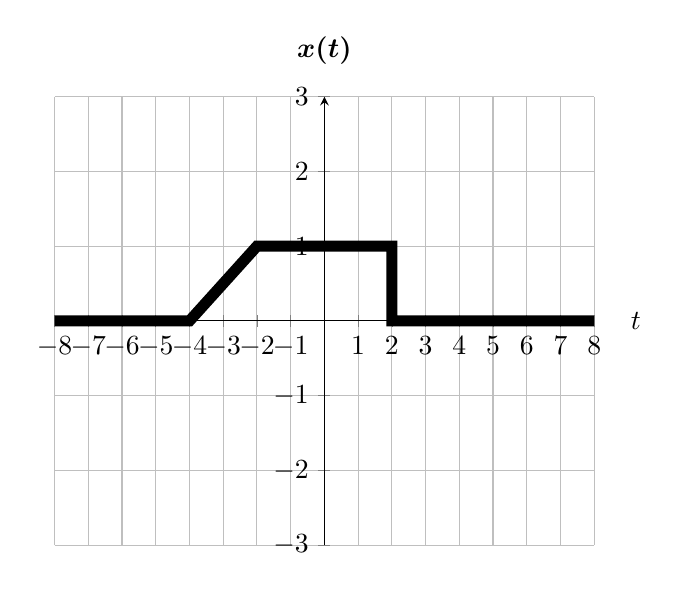
\begin{tikzpicture}[scale=1.0]
          \begin{axis}[
          axis lines=middle,
          xlabel={$t$},
          ylabel={$\boldsymbol{x(t)}$},
          xtick={-8, -7, -6, -5, -4, -3, -2, -1, ..., 8},
          ytick={-3, -2, -1, ..., 3},
          ymin=-3, ymax=3,
          xmin=-8, xmax=8,
          every axis x label/.style={at={(ticklabel* cs:1.05)}, anchor=west,},
          every axis y label/.style={at={(ticklabel* cs:1.05)}, anchor=south,},
          grid,
        ]
          \path[draw,line width=4pt] (-8,0) -- (-4,0) -- (-2,1) -- (2,1) -- (2,0) -- (6,0) -- (8,0);
          \end{axis}
        \end{tikzpicture}
        \caption{$t$ vs. $x(\frac{t}{2})$.}
        \label{fig:q2}
    \end{figure}
    
\begin{figure}[h!]
    \centering
        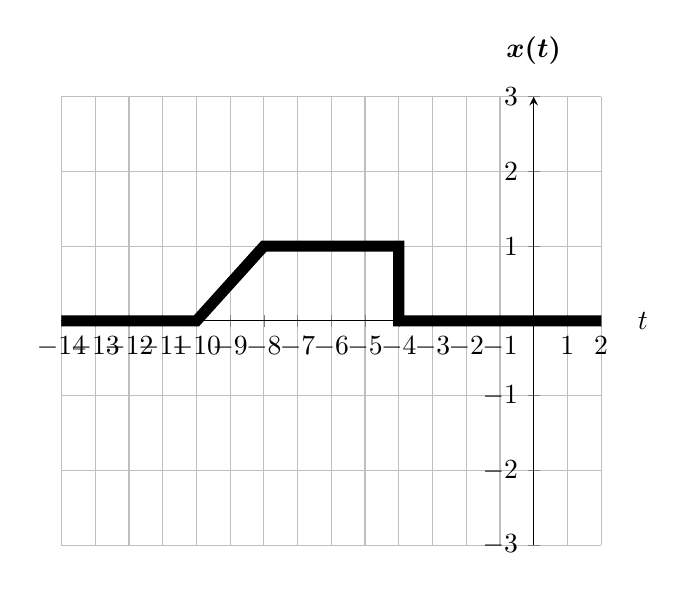
\begin{tikzpicture}[scale=1.0]
          \begin{axis}[
          axis lines=middle,
          xlabel={$t$},
          ylabel={$\boldsymbol{x(t)}$},
          xtick={-14, -13, ..., 2},
          ytick={-3, -2, -1, ..., 3},
          ymin=-3, ymax=3,
          xmin=-14, xmax=2,
          every axis x label/.style={at={(ticklabel* cs:1.05)}, anchor=west,},
          every axis y label/.style={at={(ticklabel* cs:1.05)}, anchor=south,},
          grid,
        ]
          \path[draw,line width=4pt] (-14,0) -- (-10,0) -- (-8,1) -- (-4,1) -- (-4,0) -- (0,0) -- (2,0);
          \end{axis}
        \end{tikzpicture}
        \caption{$t$ vs. $x(\frac{t}{2} + 3)$.}
        \label{fig:q2}
    \end{figure}
    
\begin{figure}[h!]
    \centering
        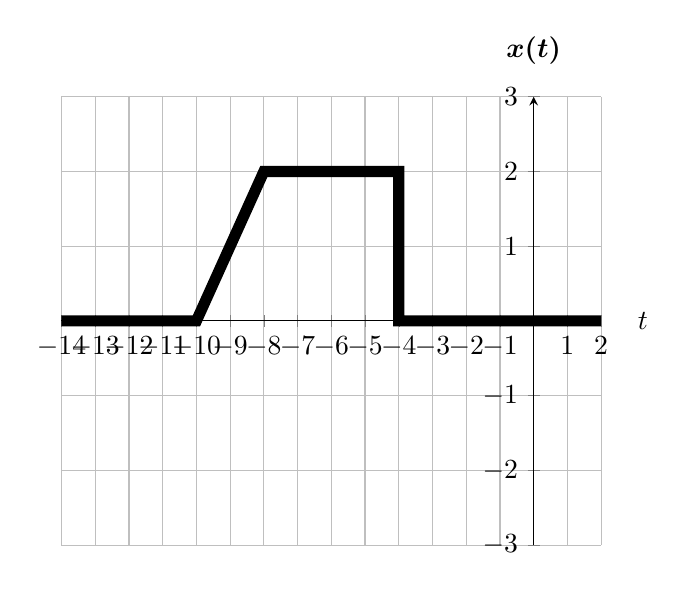
\begin{tikzpicture}[scale=1.0]
          \begin{axis}[
          axis lines=middle,
          xlabel={$t$},
          ylabel={$\boldsymbol{x(t)}$},
          xtick={-14, -13, ..., 2},
          ytick={-3, -2, -1, ..., 3},
          ymin=-3, ymax=3,
          xmin=-14, xmax=2,
          every axis x label/.style={at={(ticklabel* cs:1.05)}, anchor=west,},
          every axis y label/.style={at={(ticklabel* cs:1.05)}, anchor=south,},
          grid,
        ]
          \path[draw,line width=4pt] (-14,0) -- (-10,0) -- (-8,2) -- (-4,2) -- (-4,0) -- (0,0) -- (2,0);
          \end{axis}
        \end{tikzpicture}
        \caption{$t$ vs. $y(t) = 2x(\frac{t}{2} + 3)$.}
        \label{fig:q2}
    \end{figure}

\newpage
\item %write the solution of q4
    \begin{enumerate}

    \item Q4a\\

\begin{figure} [h!]
    \centering
    \begin{tikzpicture}[scale=1.0] 
      \begin{axis}[
          axis lines=middle,
          xlabel={$n$},
          ylabel={$\boldsymbol{x[n]}$},
          xtick={ -7, -6,  ..., 1},
          ytick={-4, -3, -2, -1, ..., 4},
          ymin=-4, ymax=4,
          xmin=-7, xmax=1,
          every axis x label/.style={at={(ticklabel* cs:1.05)}, anchor=west,},
          every axis y label/.style={at={(ticklabel* cs:1.05)}, anchor=south,},
          grid,
        ]
        \addplot [ycomb, black, thick, mark=*] table [x={n}, y={xn}] {q31.dat};
      \end{axis}
    \end{tikzpicture}
    \caption{$n$ vs. $x[-n]$.}
    \label{fig:q3}
\end{figure}

\begin{figure} [h!]
    \centering
    \begin{tikzpicture}[scale=1.0] 
      \begin{axis}[
          axis lines=middle,
          xlabel={$n$},
          ylabel={$\boldsymbol{x[n]}$},
          xtick={ -1, 0,  ..., 3},
          ytick={-4, -3, -2, -1, ..., 4},
          ymin=-4, ymax=4,
          xmin=-1, xmax=3,
          every axis x label/.style={at={(ticklabel* cs:1.05)}, anchor=west,},
          every axis y label/.style={at={(ticklabel* cs:1.05)}, anchor=south,},
          grid,
        ]
        \addplot [ycomb, black, thick, mark=*] table [x={n}, y={xn}] {q32.dat};
      \end{axis}
    \end{tikzpicture}
    \caption{$n$ vs. $x[2n+1]$.}
    \label{fig:q3}
\end{figure}

\begin{figure} [h!]
    \centering
    \begin{tikzpicture}[scale=1.0] 
      \begin{axis}[
          axis lines=middle,
          xlabel={$n$},
          ylabel={$\boldsymbol{x[n]}$},
          xtick={ -7, -6,  ..., 3},
          ytick={-4, -3, -2, -1, ..., 4},
          ymin=-4, ymax=4,
          xmin=-7, xmax=3,
          every axis x label/.style={at={(ticklabel* cs:1.05)}, anchor=west,},
          every axis y label/.style={at={(ticklabel* cs:1.05)}, anchor=south,},
          grid,
        ]
        \addplot [ycomb, black, thick, mark=*] table [x={n}, y={xn}] {q3ans.dat};
      \end{axis}
    \end{tikzpicture}
    \caption{$n$ vs. $x[-n]+x[2n+1]$.}
    \label{fig:q3}
\end{figure}

    \item $x[-n]+x[2n+1] = -4 \cdot \delta(n+7) + 3 \cdot \delta(n+4) - 2 \cdot \delta(n+2) + \delta(n+1) + \delta(n-1) - 4 \cdot \delta(n-3)$
    
    \end{enumerate} 



\item %write the solution of q5
    \begin{enumerate}
    % Write your solutions in the following items.
    \item Yes.\\
    
    $T_0 = \frac{2\pi}{7\pi} = \frac{2}{7}$
    %write the solution of q5a
    \item No.\\
    
    $T_0 = \frac{2}{4}\pi = \frac{1}{2}\pi$. Period is always a multiple of fundamental period. Since $\pi$ is irrational, there is no $T$ that is integer.
    %write the solution of q5b
    \item Yes.\\
    
    $T_{x0} = \frac{5 \cdot 2}{7} = \frac{10}{7}$\\
    
    $T_{y0} = \frac{2 \cdot 2}{5} = \frac{4}{5}$\\

    $T_0 = LCM(T_{x0}, T_{y0}) = \frac{20}{1} = 20 $\\
    %write the solution of q5c
    \end{enumerate}


\item %write the solution of q6
    \begin{enumerate}
    % Write your solutions in the following items.
    \item 
    $x(t) = x(-t)$ when $x$ is even. But $x(1.5) = 0 \not = 0.5 = x(-1.5)$. So $x$ isn't even. \\
    
    $x(t) = -x(-t)$ when $x$ is odd. But $x(1.5) = 0 \not = -0.5 = -x(-1.5)$. So $x$ isn't odd.
    
    \item ~ \\
    
\begin{figure}[h!]
    \centering
        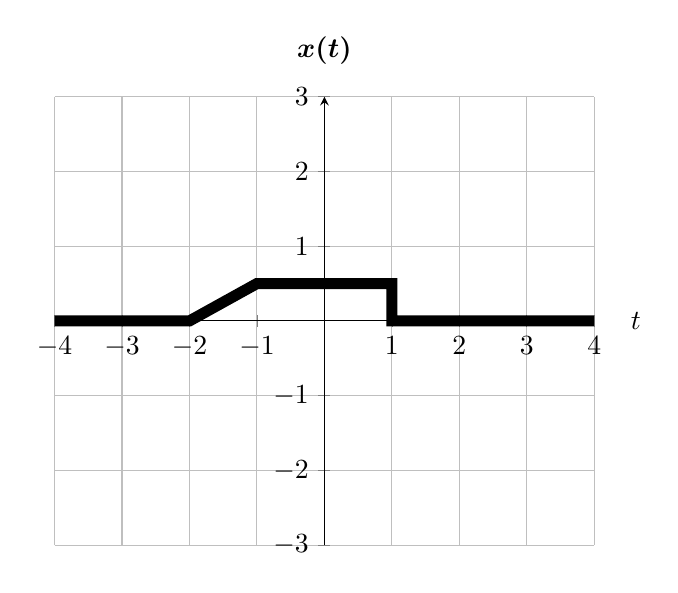
\begin{tikzpicture}[scale=1.0]
           \begin{axis}[
          axis lines=middle,
          xlabel={$t$},
          ylabel={$\boldsymbol{x(t)}$},
          xtick={-4, -3, -2, -1, ..., 4},
          ytick={-3, -2, -1, ..., 3},
          ymin=-3, ymax=3,
          xmin=-4, xmax=4,
          every axis x label/.style={at={(ticklabel* cs:1.05)}, anchor=west,},
          every axis y label/.style={at={(ticklabel* cs:1.05)}, anchor=south,},
          grid,
        ]
           \path[draw,line width=4pt] (-4,0) -- (-2,0) -- (-1,0.5) -- (1,0.5) -- (1,0) -- (3,0) -- (4,0);
           \end{axis}
        \end{tikzpicture}
        \caption{$t$ vs. $\frac{1}{2} \cdot x(t)$.}
        \label{fig:q2}
    \end{figure}
    
\begin{figure}[h!]
    \centering
        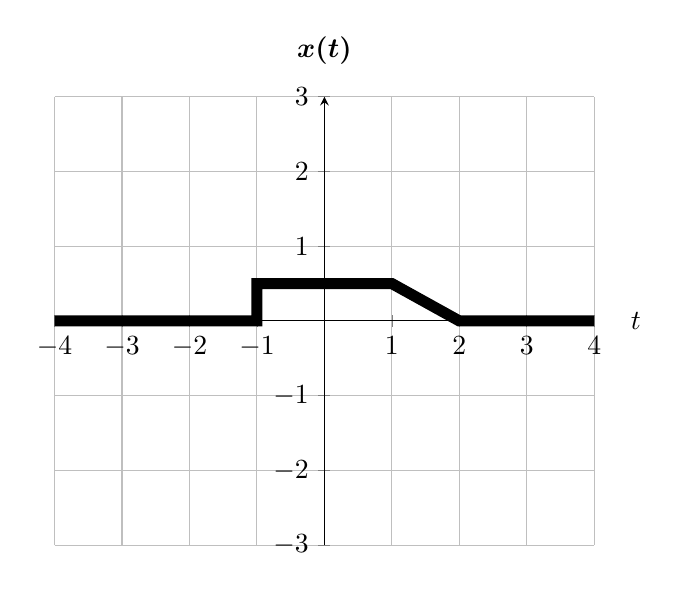
\begin{tikzpicture}[scale=1.0]
           \begin{axis}[
          axis lines=middle,
          xlabel={$t$},
          ylabel={$\boldsymbol{x(t)}$},
          xtick={-4, -3, -2, -1, ..., 4},
          ytick={-3, -2, -1, ..., 3},
          ymin=-3, ymax=3,
          xmin=-4, xmax=4,
          every axis x label/.style={at={(ticklabel* cs:1.05)}, anchor=west,},
          every axis y label/.style={at={(ticklabel* cs:1.05)}, anchor=south,},
          grid,
        ]
           \path[draw,line width=4pt] (4,0) -- (2,0) -- (1,0.5) -- (-1,0.5) -- (-1,0) -- (-3,0) -- (-4,0);
           \end{axis}
        \end{tikzpicture}
        \caption{$t$ vs. $\frac{1}{2} \cdot x(-t)$.}
        \label{fig:q2}
    \end{figure}
    
\begin{figure}[h!]
    \centering
        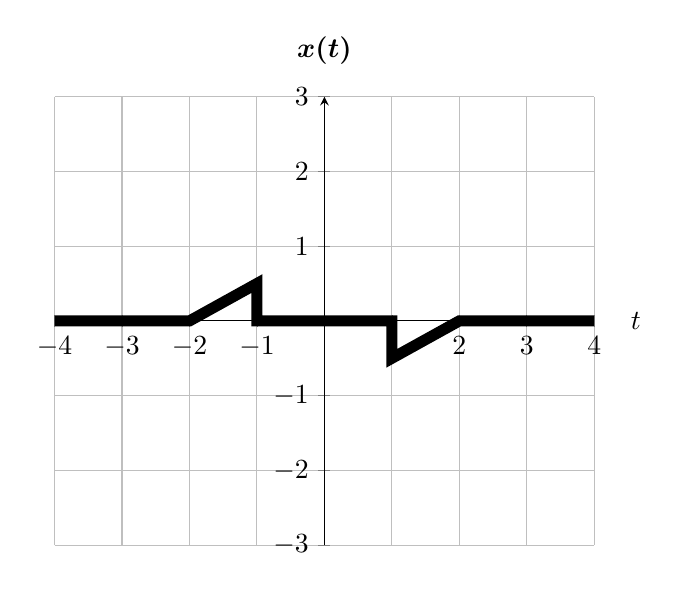
\begin{tikzpicture}[scale=1.0]
           \begin{axis}[
          axis lines=middle,
          xlabel={$t$},
          ylabel={$\boldsymbol{x(t)}$},
          xtick={-4, -3, -2, -1, ..., 4},
          ytick={-3, -2, -1, ..., 3},
          ymin=-3, ymax=3,
          xmin=-4, xmax=4,
          every axis x label/.style={at={(ticklabel* cs:1.05)}, anchor=west,},
          every axis y label/.style={at={(ticklabel* cs:1.05)}, anchor=south,},
          grid,
        ]
           \path[draw,line width=4pt] (-4,0) -- (-2,0) -- (-1,0.5) -- (-1,0) -- (1,0) -- (1,-0.5) -- (2,0) -- (3,0) -- (4,0);
           \end{axis}
        \end{tikzpicture}
        \caption{$t$ vs. $Odd\{x(t)\} = \frac{1}{2}(x(t) - x(-t))$.}
        \label{fig:q2}
    \end{figure}
\newpage

\begin{figure}[h!]
    \centering
        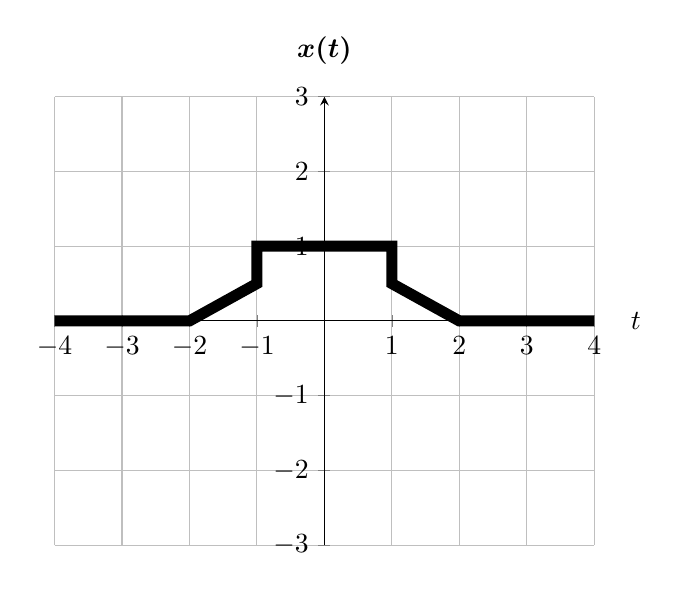
\begin{tikzpicture}[scale=1.0]
           \begin{axis}[
          axis lines=middle,
          xlabel={$t$},
          ylabel={$\boldsymbol{x(t)}$},
          xtick={-4, -3, -2, -1, ..., 4},
          ytick={-3, -2, -1, ..., 3},
          ymin=-3, ymax=3,
          xmin=-4, xmax=4,
          every axis x label/.style={at={(ticklabel* cs:1.05)}, anchor=west,},
          every axis y label/.style={at={(ticklabel* cs:1.05)}, anchor=south,},
          grid,
        ]
           \path[draw,line width=4pt] (-4,0) -- (-2,0) -- (-1,0.5) -- (-1,1) -- (1,1) -- (1,0.5) -- (2,0) -- (3,0) -- (4,0);
           \end{axis}
        \end{tikzpicture}
        \caption{$t$ vs. $Even\{x(t)\} = \frac{1}{2}(x(t) + x(-t))$.}
        \label{fig:q2}
    \end{figure}
    
    %write the solution of q6b
    \end{enumerate}

\newpage 

\item %write the solution of q7
    \begin{enumerate}
    % Write your solutions in the following items.
    \item %write the solution of q7a 
    $x(t) = -3u(t-2) + 5u(t-3) - 3u(t-5)$ \\
    \item %write the solution of q7b
    $\frac{du(t)}{dt} = \delta(t)$ \\ 
    
    $\frac{dx(t)}{dt} = -3\delta(t-2)+5\delta(t-3)-3\delta(t-5)$ \\
    
\begin{figure}[h!]
        \centering
        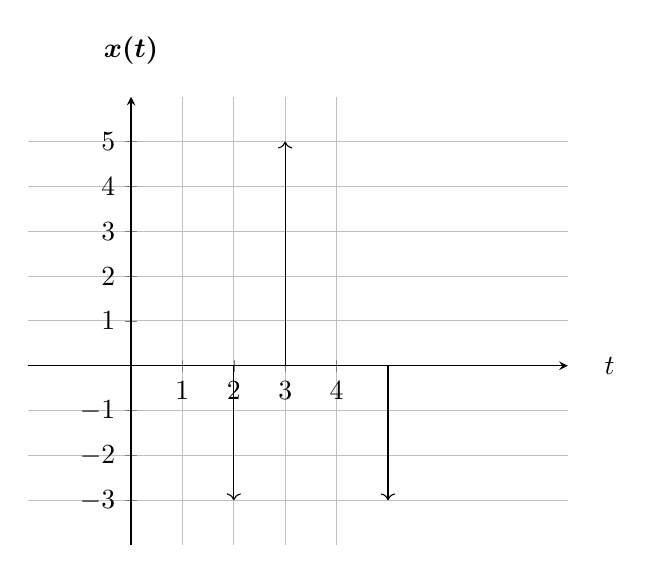
\begin{tikzpicture}[scale=1.0]
           \begin{axis}[
          axis lines=middle,
          xlabel={$t$},
          ylabel={$\boldsymbol{x(t)}$},
          xtick={0, 1, ..., 4},
          ytick={-3, -2, -1, 0, 1, 2, 3, ..., 5},
          ymin=-4, ymax=6,
          xmin=-2, xmax=8.5,
          every axis x label/.style={at={(ticklabel* cs:1.05)}, anchor=west,},
          every axis y label/.style={at={(ticklabel* cs:1.05)}, anchor=south,},
          grid,
        ]
           \draw [->] (2,0) -- (2,-3);
           \draw [->] (3,0) -- (3,5);
           \draw [->] (5,0) -- (5,-3);
           \end{axis}
        \end{tikzpicture}
        \caption{$t$ vs. $\frac{dx(t)}{dt}$.}
        \label{fig:q6}
    \end{figure}
    
    \end{enumerate}    

\item %write the solution of q8
    \begin{enumerate}
    % Write your solutions in the following items.
    \item 
        \begin{enumerate}
        \item Memory: Yes. $3n-5 \not = n $
        \item Stability: Yes, bounded inputs always generate bounded outputs.
        \item Causality: No. When $n>2$, it doesn't satisfy causality. $n=3, 3*(3) - 5 > (3)$
        \item Linearity: Yes, it satisfies both superposition and homogeneity.
        \item Invertibility: Yes, for $h^{-1}[n] = \frac{n + 5}{3}$.
        \item Time-invariance: Yes, $y[n - n_0] = x[3(n - n_0) - 5]$.
        \end{enumerate}
    %write the solution of q8a
    \item
        \begin{enumerate}
        \item Memory: Yes. $3t-5 \not = t $
        \item Stability: Yes, bounded inputs always generate bounded outputs.
        \item Causality: No. When $t \geq 3$, it doesn't satisfy causality. $n=3, 3 \cdot (3) - 5 > (3)$
        \item Linearity: Yes, it satisfies both superposition and homogeneity.
        \item Invertibility: Yes, for $h^{-1}(t) = \frac{t + 5}{3}$.
        \item Time-invariance: Yes, $y(n - n_0) = x(3(n - n_0) - 5)$.
        \end{enumerate}
    %write the solution of q8b
    \item 
        \begin{enumerate}
        \item Memory: Yes. $t-1 \not = t $
        \item Stability: No, the bounded input does not always generate a bounded output. 
        \item Causality: Yes, $t-1$ is less than $t$.
        \item Linearity: Yes, it satisfies both superposition and homogeneity.
        \item Invertibility: No, for $t = 0$ the system is not invertible.
        \item Time-invariance: No, $y(t - t_0) = (t - t_0) \cdot x((t - t_0) - 1) \not = t \cdot x((t - t_0) - 1)$.
        \end{enumerate}%write the solution of q8c
    \item 
        \begin{enumerate}
        \item Memory: Yes. $n-k \not = n $ when $k>1$.
        \item Stability: No, the sum is an infinity sum.
        \item Causality: Yes, $n-k$ is always less than $n$.
        \item Linearity: Yes, it satisfies both superposition and homogeneity.
        \item Invertibility: No. % TODO %
        \item Time-invariance: Yes, $y[n - n_0] = \sum_{k  =1}^{\infty} x[(n - n_0) - k]$.
        \end{enumerate}%write the solution of q8d
    \end{enumerate}
    
    Please note that:
    \begin{itemize}
        \item Let $y(t) = h(x(t))$, $y_1(t) = h(x_1(t))$, and $y_2(t) = h(x_2(t))$.
        \item Superposition means that $y_1(t) + y_2(t) = h(x_1(t) + x_2(t))$.
        \item Homogeneity means that for a arbitrary $k$, $k \cdot y(t) = h(k \cdot x(t))$.
    \end{itemize}
    
\end{enumerate}
\end{document}

